% section7

\chapter{Dimension and Structure}

\section{Basis and Dimension}

\begin{exer} (\textit{Linear Combination and Independence})\\
Are any of the vectors in the set
\vspace{1mm}
\begin{displaymath}
S = \{ (2,6,3,4,2), \hspace{1.5mm}(3,1,5,8,3), \hspace{1.5mm}(5,1,2,6,7), \hspace{1.5mm}(8,4,3,2,6), \hspace{1.5mm}(5,5,6,3,4) \}
\end{displaymath}
\vspace{1mm}
linear combinations of predecessors? Justify your answer.

\end{exer}


\begin{sol}
\verb""
One strategy is to form a matrix $V$ of the column vectors $\mathbf{v}_{k}$ mentioned above and decide whether the system $V \mathbf{x} = \mathbf{0}$ has nontrivial solutions. If so, then at least one column is a linear combination of previous ones. Otherwise, the columns are linearly independent.

\begin{verbatim}

v1 = [2 6 3 4 2]'; v2 = [3 1 5 8 3]'; v3 = [5 1 2 6 7]';
v4 = [8 4 3 2 6]'; v5 = [5 5 6 3 4]';

% Construct V of the column vectors v1,v2,v3,v4 and v5.
V = [v1 v2 v3 v4 v5]; 

format short;

% Find the reduced row echelon form of V.
rref_V = rref(V); 

disp('The reduced row echelon form of A is'); disp(rref_V);
\end{verbatim}



\begin{outputs}

\begin{verbatim}

The reduced row echelon form of A is
     1     0     0     0     0
     0     1     0     0     0
     0     0     1     0     0
     0     0     0     1     0
     0     0     0     0     1
\end{verbatim}

\end{outputs}



\noindent Since the reduced row echelon form of $V$ has 5 pivots, the columns of V are linearly independent. Hence, no column of $V$ can be a linear combination of any other columns.
\end{sol}

\vspace{2mm}

\section{Properties of Bases}


\begin{exer}
In this problem, we make a function file \verb"CheckBasis.m" to check that the vectors $\mathbf{v}_{1}$, $\mathbf{v}_{2}$, $\mathbf{v}_{3}$ and $\mathbf{v}_{4}$ form a basis of $\mathbb{R}^4$ using the equivalent statements (a), (g), (h), and (o) of Theorem 7.2.7 in the textbook.

\begin{enumerate}
\item[(a)]
Complete the shadow part (/////) of the m-file given below referring to the comments and the execution results.

\begin{verbatim}

%--- your function file ---%
function [Result]=CheckBasis(v1, v2, v3, v4, case_num)
  %  if case_num=1, check the statement (a),
  %  if case_num=2, check the statement (g),
  %  if case_num=3, check the statement (h).

  % Construct the matrix V.
  ////////////////////////

  % Use the switch statement to check 
  % whether one of the statements (a), (g), and (h) holds.
  switch case_num
    case 1  
      fprintf('* You enter %d: statement (a) *\n', case_num);
      ////////////////////////
      if ////////////////////////
        disp('Given vectors form a basis of 4 dimensional space.');
      else
        disp('Given vectors do not form a basis of 4 dimensional space.');
      end
    case 2
      fprintf('* You enter %d: statement (g) *\n', case_num);
      Result=det(V);
      if Result~=0
        disp('Given vectors form a basis of 4 dimensional space.');
      else
        disp('Given vectors do not form a basis of 4 dimensional space.');
      end
    ///////////////////////////  % check statement (h)
        ////////////////////////
        ////////////////////////
        ////////////////////////
        ////////////////////////
        ////////////////////////
        ////////////////////////
        ////////////////////////
  end
end
\end{verbatim}

\vspace{3mm}

\noindent The execution results will be as follows:
\begin{verbatim}
>> v1=[1 0 0 0]'; v2=[0 2 0 0]'; v3=[0 0 4 5]'; v4=[0 0 0 -1]'; v5=[0 0 0 1]';
>> C=CheckBasis(v1, v2, v3, v4,3)
* You enter 3: statement (h) *
  Given vectors are basis of 4 dimensional space.

C =

     1
     2
    -1
     4

>> CheckBasis(v1, v2, v4, v5, 1);
* You enter 1: statement (a) *
  Given vectors do not form a basis of 4 dimensional space.

>> determinant=CheckBasis(v1, v2, v3, v5, 2)
* You enter 2: statement (g) *
  Given vectors form a basis of 4 dimensional space.

determinant =
     8
\end{verbatim}

\vspace{3mm}
\item[(b)] Using \verb"CheckBasis.m" from (a), check whether
\begin{itemize}
\item[i.] $\mathbf{v}_{1}=(-1, 0, 1, 0)^{T}$, $\mathbf{v}_{2}=(2, 3, -2, 6)^{T}$, $\mathbf{v}_{3}=(0, -1, 2, 0)^{T}$ and $\mathbf{v}_{4}=(0, 0, 1, 5)^{T}$ form a basis of $\mathbb{R}^4$.

\item[ii.] $\mathbf{v}_{1}=(a, b, c, d)^{T}$, $\mathbf{v}_{2}=(-b, a, d, -c)^{T}$, $\mathbf{v}_{3}=(-c, -d, a, b)^{T}$ and $\mathbf{v}_{4}=(-d, c, -b, a)^{T}$ form a basis of $\mathbb{R}^4$. (Do not use the statement (h). Guess why not?)
\end{itemize}

\end{enumerate}
\end{exer}


\begin{sol}

\vspace{1mm}
\verb""
\begin{enumerate}
\item[(a)]
\verb" "
\verb"% ----- your function file ----- %"\\
\verb"function [Result]=CheckBasis(v1, v2, v3, v4, case_num)"\\
\verb"  %  if case_num=1, check the statement (a),"\\
\verb"  %  if case_num=2, check the statement (g),"\\
\verb"  %  if case_num=3, check the statement (h)."\\
\\
\verb" % Construct the matrix V."\\
  \textcolor{blue}{\texttt{  V=[v1 v2 v3 v4];}}\\

\verb"  % Use the switch statement to check" \\
\verb"  % whether one of the statements (a), (g), and (h) holds."\\
\verb"  switch case_num"\\
\verb"    case 1"  \\
\verb"      fprintf('* You enter %d: statement (a) *', case_num);"\\
\textcolor{blue}{\texttt{ \hspace{8mm}         Result=rref(V)}}

\hspace{8mm}      \texttt{ if \textcolor{blue}{det(Result)$\sim$=0}}\\
\verb"        disp('Given vectors form a basis of 4 dimensional space.');"\\
\verb"      else"\\
\verb"        disp('Given vectors do not form a basis of 4 dimensional space.');"\\
\verb"      end"\\
\verb"    case 2"\\
\verb"      fprintf('* You enter %d: statement (g) *', case_num);"\\
\verb"      Result=det(V);"\\
\verb"      if Result~=0"\\\
\verb"        disp('Given vectors form a basis of 4 dimensional space.');"\\
\verb"      else"\\
\verb"        disp('Given vectors do not form a basis of 4 dimensional space.');"\\
\verb"      end"\\
\textcolor{blue}{\texttt{  \hspace{4mm}  case 3}}\verb"  % check statement (h)"\\
\textcolor{blue}{\texttt{  \hspace{8mm}      [Q D]=eig(V);}}

\textcolor{blue}{\texttt{  \hspace{8mm}            Result=diag(R);}}

\textcolor{blue}{\texttt{  \hspace{8mm}         if det(R)==0}}

\textcolor{blue}{\texttt{   \hspace{12mm}       disp('Given vectors form a basis of 4 dimensional space.');}}

\textcolor{blue}{\texttt{  \hspace{8mm}              else}}

 \textcolor{blue}{\texttt{  \hspace{12mm}               disp('Given vectors do not form a basis of 4 dimensional space.');}}

\textcolor{blue}{\texttt{  \hspace{8mm}        end}}

\textcolor{blue}{\texttt{  \hspace{4mm}      end}}


\item[(b)-i.] 
\begin{verbatim}
>> v1=[-1 0 1 0]'; v2=[2 3 -2 6]';  v3=[0 -1 2 0]'; v4 = [0 0 1 5]';
>> CheckBasis(v1, v2, v3, v4, 1);
>> CheckBasis(v1, v2, v3, v4, 2);
>> CheckBasis(v1, v2, v3, v4, 3);
\end{verbatim}

\begin{outputs}
\begin{verbatim}

* You enter 1: statement (a) *
  Given vectors form a basis of 4 dimensional space.
* You enter 2: statement (g) *
  Given vectors form a basis of 4 dimensional space.
* You enter 3: statement (h) *
  Given vectors form a basis of 4 dimensional space.
\end{verbatim}
\end{outputs}

\item[(b)-ii.] 
\begin{verbatim}
>> syms a b c d;
>> v1=[a;b;c;d]; v2=[-b;a;d;-c]; v3=[-c;-d;a;b]; v4 = [-d;c;-b;a];
>> CheckBasis(v1, v2, v3, v4, 1);
>> CheckBasis(v1, v2, v3, v4, 2);
\end{verbatim}

\begin{outputs}
\begin{verbatim}

* You enter 1: statement (a) *
  Given vectors form a basis of 4 dimensional space.
* You enter 2: statement (g) *
  Given vectors form a basis of 4 dimensional space.
\end{verbatim}
\end{outputs}
\end{enumerate}
\end{sol}



\section{The Fundamental Spaces of a Matrix}


\begin{exer}\label{ex1}
In this problem, we make a function file \verb"getFSinfo.m" to get the dimension and basis of the fundamental spaces of a given matrix. For example, we execute the followings:
\begin{verbatim}
>> A=[1 0 0 0 2; -2 1 -3 -2 -4; 0 5 -14 -9 0; 2 10 -28 -18 4];
>> getFSinfo(A);
\end{verbatim}
Then, the Command Window displays the results as follows:
\begin{verbatim}
Given matrix is:
     1     0     0     0     2
    -2     1    -3    -2    -4
     0     5   -14    -9     0
     2    10   -28   -18     4

== Dimension of the fundamental spaces of a given matrix ==
dim(row(A))=dim(col(A)): 3, 	 dim(null(A)): 2, 	 dim(null(A_trans)): 1

== Basis of the fundamental spaces of a given matrix (in row vectors) ==
 row(A)
     1     0     0     0     2
     0     1     0     1     0
     0     0     1     1     0

 col(A)
     1     0     0     2
     0     1     0     0
     0     0     1     2

 null(A)
     0    -1    -1     1     0
    -2     0     0     0     1

 null(A_trans)
    -2     0    -2     1

*****************************************************
\end{verbatim}
\begin{enumerate}
\item[(a)] Complete the missing parts of the m-file \verb"getFSinfo" given as follows:
\begingroup
    \fontsize{10pt}{12pt}\selectfont
\begin{verbatim}

%--- function file 'getFSinfo.m' ---%
function [info]=getFSinfo(A)
  % row(A): basis and dimension
  /////// missing part ///////

  % col(A): basis and dimension
  /////// missing part ///////

  % null(A): basis and dimension
  /////// missing part ///////

  % null(A'): basis and dimension
  /////// missing part ///////

  disp('Given matrix is:'); disp(A);
  fprintf('== Dimension of the fundamental spaces of given matrix == \n');
  fprintf('dim(row(A))=dim(col(A)): %d,', rank_A);
  fprintf('\t dim(null(A)): %d,\t dim(null(A_trans)): %d \n\n', nullity, nullity_T);
  fprintf('== Basis of the fundamental spaces of given matrix (in row vectors) == \n');
  disp(' row(A)'); disp(double(rowA_basis));
  disp(' col(A)'); disp(double(colA_basis));
  disp(' null(A)'); disp(nullA_basis);
  disp(' null(A_trans)'); disp(nullAtrans_basis);
  fprintf('\n*****************************************************\n');
end
\end{verbatim}
\endgroup
You may use the MATLAB commands \textit{rank, colspace, rref, null} and so on.
\vspace{3mm}
\item[(b)] Using your function file \verb"getFSinfo.m", find the dimension and basis of the fundamental spaces of

$A = \begin{bmatrix} 3 & 2& 1& 3& 5 \\ 6& 4& 3& 5& 7 \\ 9&6&5&7&9\\3&2&0&4&8 \end{bmatrix}$, $B = \begin{bmatrix} 3 & -1 & 3& 2& 5 \\ 5& -3&2&3&4\\ 1&-3&-5&0& -7\\ 7&-5&1&4&1\end{bmatrix}$, $C = \begin{bmatrix} 1& 3& 2& 1\\ -2 & -6 & 0& -6\\ 3& 9& 1& 8\\ -1& -3& -3& -6\\ 1& 3& 2& 1\\ 4& 12& 1&11 \end{bmatrix}$.
\end{enumerate}
\end{exer}

\begin{sol}
\verb""
\begin{enumerate}
\item[(a)]

\verb"% ----- function file 'getFSinfo.m' ----- %"

\verb"function [info]=getFSinfo(A)"

\verb"  [m,n]=size(A)"

\verb"  % row(A): basis and dimension"

{\color{blue}\verb"    rank_A=rank(A);    % rank of A;"

    \verb"    rowA=colspace(sym(A')); % find the row basis"

    \verb"    rowA_basis=rowA(:, 1:rank_A)';  % basis of row(A)"
    }



\verb"  % col(A): basis and dimension"

{\color{blue}\verb"    colA=colspace(sym(A)); % find the column basis"

\verb"    colA_basis=colA(:, 1:rank_A)';  % basis of col(A)"
    }




\verb"  % null(A): basis and dimension"

{\color{blue}\verb"    nullA=null(A, 'r');"

\verb"    nullity=n-rank_A;   % using Dimension theorem"

\verb"    nullA_basis=nullA(:, 1:nullity)';"
    }

\verb"  % null(A'): basis and dimension"

{\color{blue}\verb"    nullAtrans=null(A', 'r');"

    \verb"    nullity_T=m-rank_A;    "

    \verb"    nullAtrans_basis=nullAtrans(:,1:nullity_T)';"
    }
\begin{verbatim}
  disp('Given matrix is:'); disp(A);
  fprintf('== Dimension of the fundamental spaces of given matrix == \n');
  fprintf('dim(row(A))=dim(col(A)): %d,', rank_A);
  fprintf('\t dim(null(A)): %d,', nullity);
  fprintf('\t dim(null(A_trans)): %d \n\n', nullity_T);
  fprintf('== Basis of the fundamental spaces ');
  fprintf('of given matrix (in row vectors) == \n');
  disp(' row(A)'); disp(double(rowA_basis));
  disp(' col(A)'); disp(double(colA_basis));
  disp(' null(A)'); disp(nullA_basis);
  disp(' null(A_trans)'); disp(nullAtrans_basis);
  fprintf('\n*****************************************************\n');
end
\end{verbatim}

\item[(b)]
\begin{verbatim}
A=[3 2 1 3 5; 6 4 3 5 7; 9 6 5 7 9; 3 2 0 4 8];
B=[3 -1 3 2 5; 5 -3 2 3 4; 1 -3 -5 0 -7; 7 -5 1 4 1];
C=[1 3 2 1; -2 -6 0 -6 ;3 9 1 8; -1 -3 -3 -6; 1 3 2 1; 4 12 1 11];
getFSinfo(A);
getFSinfo(B);
getFSinfo(C);
\end{verbatim}


\begin{outputs}
\begin{verbatim}

Given matrix is:
     3     2     1     3     5
     6     4     3     5     7
     9     6     5     7     9
     3     2     0     4     8
== Dimension of the fundamental spaces of given matrix ==
dim(row(A))=dim(col(A)): 2,	 dim(null(A)): 3,	 dim(null(A_trans)): 2
== Basis of the fundamental spaces of given matrix (in row vectors) ==
 row(A)
    1.0000    0.6667         0    1.3333    2.6667
         0         0    1.0000   -1.0000   -3.0000
 col(A)
     1     0    -1     3
     0     1     2    -1
 null(A)
   -0.6667    1.0000         0         0         0
   -1.3333         0    1.0000    1.0000         0
   -2.6667         0    3.0000         0    1.0000
 null(A_trans)
     1    -2     1     0
    -3     1     0     1
*****************************************************

Given matrix is:
     3    -1     3     2     5
     5    -3     2     3     4
     1    -3    -5     0    -7
     7    -5     1     4     1
== Dimension of the fundamental spaces of given matrix ==
dim(row(A))=dim(col(A)): 3,	 dim(null(A)): 2,	 dim(null(A_trans)): 1
== Basis of the fundamental spaces of given matrix (in row vectors) ==
 row(A)
    1.0000         0    1.7500    0.7500         0
         0    1.0000    2.2500    0.2500         0
         0         0         0         0    1.0000
 col(A)
     1     0    -3     0
     0     1     2     0
     0     0     0     1
 null(A)
   -1.7500   -2.2500    1.0000         0         0
   -0.7500   -0.2500         0    1.0000         0
 null(A_trans)
     3    -2     1     0
*****************************************************

Given matrix is:
     1     3     2     1
    -2    -6     0    -6
     3     9     1     8
    -1    -3    -3    -6
     1     3     2     1
     4    12     1    11
== Dimension of the fundamental spaces of given matrix ==
dim(row(A))=dim(col(A)): 3,	 dim(null(A)): 1,	 dim(null(A_trans)): 3
== Basis of the fundamental spaces of given matrix (in row vectors) ==
 row(A)
     1     3     0     0
     0     0     1     0
     0     0     0     1
 col(A)
    1.0000         0    0.5000         0    1.0000    0.5000
         0    1.0000   -1.2500         0         0   -1.7500
         0         0         0    1.0000         0         0
 null(A)
    -3     1     0     0
 null(A_trans)
   -0.5000    1.2500    1.0000         0         0         0
   -1.0000         0         0         0    1.0000         0
   -0.5000    1.7500         0         0         0    1.0000
*****************************************************
\end{verbatim}
\end{outputs}
\end{enumerate}
\end{sol}

\vspace{3mm}

\begin{exer}
(\textit{Bases for the Fundamental Spaces})

\begin{enumerate}

\item[(a)] Use the MATLAB commands \textit{sym} and \textit{colspace} to find a basis for the column space of the matrix

\begin{displaymath}
A = \left[\begin{array}{rrrr} 2& \hspace{2mm} -1& \hspace{5mm} 3&\hspace{4mm} 5\\ 4 & -3 & 1 & 3 \\ 3 & -2 & 3 & 4 \\ 4 & -1 & 15 & 17 \\ 7 & -6 & -7 & 0 \end{array} \right].
\end{displaymath}

\vspace{1mm}

\item[(b)] Use the same MATLAB commands in (a) to find a basis for the row space of $A$.

\vspace{1mm}

\item[(c)] Confirm that the basis obtained in (b) is consistent with the basis obtained from the reduced row echelon form of $A$.

\vspace{1mm}

\item[(d)] Tell what happens if you use the MATLAB command \textit{orth}?

\end{enumerate}
\end{exer}



\begin{sol}
\verb""

%\vspace{3mm}


\begin{itemize}
\item[(a)]
\begin{verbatim}
% Set a matrix A whose entries are symbolic objects.
A = sym([2 -1 3 5; 4 -3 1 3; 3 -2 3 4; 4 -1 15 17; 7 -6 -7 0]);

% Find a basis for the column space of A.
col_basis = colspace(A);

disp('A basis for the column space of A is');
disp(col_basis(:,1)'); disp(col_basis(:,2)'); disp(col_basis(:,3)');
\end{verbatim}


\begin{outputs}
\begin{verbatim}

A basis for the column space of A is
[ 1, 0, 0, 2, 1]

[ 0, 1, 0, -3, 5]

[ 0, 0, 1, 4, -5]
\end{verbatim}
\end{outputs}


\item[(b)]
\begin{verbatim}
% Set a matrix A_transpose whose entries are symbolic objects.
A_transpose = sym([2 -1 3 5; 4 -3 1 3; 3 -2 3 4; 4 -1 15 17; 7 -6 -7 0]');

% Finding a basis for the row space of A is equivalent to
% finding a basis for the column space of A_transpose.
rowbasis = colspace(A_transpose);

disp('A basis for the row space of A is');
disp(rowbasis(:,1)'); disp(rowbasis(:,2)'); disp(rowbasis(:,3)');
\end{verbatim}



\begin{outputs}
\begin{verbatim}

A basis for the row space of A is
[ 1, 0, 0, 6]

[ 0, 1, 0, 7]

[ 0, 0, 1, 0]
\end{verbatim}
\end{outputs}



\item[(c)]
\begin{verbatim}
% Set a matrix A.
A = [2 -1 3 5; 4 -3 1 3; 3 -2 3 4; 4 -1 15 17; 7 -6 -7 0];

% Find the reduced row echelon form of A.
rref_A = rref(A); 

% The nonzero rows of the reduced row echelon form of A
% form a basis for the row space of A.

disp('A basis for the row space of A is');
disp(rref_A(1,:)); disp(rref_A(2,:)); disp(rref_A(3,:));
\end{verbatim}

\begin{outputs}
\begin{verbatim}

A basis for the row space of A is
     1     0     0     6

     0     1     0     7

     0     0     1     0
\end{verbatim}
\end{outputs}

\item[(d)]

\begin{verbatim}
% Set A.
A = [2 -1 3 5; 4 -3 1 3; 3 -2 3 4; 4 -1 15 17; 7 -6 -7 0]; 

% The command orth gives an orthonormal basis for the column space of A.
B = orth(A);

disp('An orthonormal basis for the column space of A is');
disp('q1='); disp(B(:,1)');
disp('q2='); disp(B(:,2)');
disp('q3='); disp(B(:,3)');
\end{verbatim}

\begin{outputs}
\begin{verbatim}

An orthonormal basis for the column space of A is
q1=
   -0.2427   -0.1508   -0.2229   -0.9246    0.1177

q2=
   -0.1189   -0.3624   -0.2060    0.0253   -0.9008

q3=
    0.3760   -0.6016   -0.5930    0.1848    0.3331
\end{verbatim}
\end{outputs}
\end{itemize}
\end{sol}

\section{The Dimension Theorem and Its Implications}


\begin{exer}
(\textit{Rank and Nullity})

\begin{enumerate}

\item[(a)] Use the MATLAB command \textit{rank} and the Formula (2) in Section $7.4$ to find the nullity of the matrix

\begin{displaymath}
A = \left[\begin{array}{rrrrr} 3& \hspace{1mm} 2& \hspace{1mm} 1&\hspace{1mm} 3&\hspace{1mm} 5\\ 6 & 4 & 3 & 5 & 7 \\ 9 & 6 & 5 & 7 & 9 \\ 3 & 2 & 0 & 4 & 8 \end{array} \right].
\end{displaymath}


\item[(b)] Confirm that the result obtained in (a) is consistent with the number of basis vectors which are obtained by using the MATLAB command \textit{null}.

\end{enumerate}

\end{exer}


\begin{sol}
\verb""
\begin{itemize}


\item[(a)]

\begin{verbatim}
% Set A.
A = [3 2 1 3 5; 6 4 3 5 7; 9 6 5 7 9; 3 2 0 4 8]; 

% Find the rank of A by using the command rank.
rank_A = rank(A); 

% Size of the matrix A.
[ m n ] = size(A); 
% m = the number of rows of A, n = the number of columns of A.

 % By (2) in section 7.4, rankA + nullA = n.
null_A = n - rank_A;

disp('The nullity of A is'); disp(null_A);
\end{verbatim}

\begin{outputs}
\begin{verbatim}

The nullity of A is
     3
\end{verbatim}
\end{outputs}


\item[(b)]
\begin{verbatim}
% Set A.
A = [3 2 1 3 5; 6 4 3 5 7; 9 6 5 7 9; 3 2 0 4 8]; 

% Find a basis for the null space of A.
nullA = null(A,'r'); 
% null(A,'r') returns a matrix 
% whose columns are a basis for the null space of A.

[m n] = size(nullA);
% Since the number of columns of nullA is n,
% thus, n = the number of basis vectors of the null space of A.

disp('The nullity of A is'); disp(n);
\end{verbatim}


\begin{outputs}
\begin{verbatim}

The nullity of A is
     3
\end{verbatim}
\end{outputs}





\end{itemize}

\end{sol}




\section{The Rank Theorem and Its Implications}

\begin{exer}
Note that the rank of a nonzero matrix $A$ is equal to the order of the largest square submatrix of $A$ (formed by deleting rows and columns of $A$) whose determinant is nonzero. In this problem, we make a function file \verb"CheckRank.m" to find the rank of the given matrix using this fact. We want to obtain the execution results as follows:
\begin{verbatim}
>> A=[1 2 3 4; 5 6 7 8; 9 10 11 12; 13 14 15 16];
>> rankA=CheckRank(A)
rankA =
     2
\end{verbatim}
For this, you may start with the largest square matrices to be found in $A$ and a search is started for the first submatrix with a nonzero determinant. Use the MATLAB command \textit{nchoosek} to select all the combinations of rows and columns needed in the search process and you may use the several MATLAB commands if you need. Complete the m-file below and check the determinant of the matrices $A$, $B$, and $C$ given in the Exercise \ref{ex1} (b). Also, compare the results using the MATLAB command \textit{rank}.
\end{exer}


\begin{sol}
\begin{verbatim}

%--- function file 'CheckRank.m' ---%
function [rank_A]= CheckRank(A)
\end{verbatim}

{\color{blue}
\begin{verbatim}
    [m,n]=size(A);  % size of given matrix
    flg=1;  % flag for while loop
    if m>n  % if (# of row) > (# of col)
        A=A';
    end
    A=sym(A);   % Set A as a symbolic object

    K = min(m,n);   N = max(m,n);   % k : row number, N: col number
    k=K;    % from the largest size of submatrix
    while flg == 1
        comb_row=nchoosek(1:K, k);  % combinations of row
        comb_col=nchoosek(1:N, k);  % combinations of columns
        for ii=1:size(comb_row) %
            selected_A=A(comb_row(ii,:),:); % selected row index
            for jj=1:size(comb_col)
                sub_A=selected_A(:,comb_col(jj, :));   % selected col index
                if det(sub_A)~=0    % if non zeros determinant appears
                    rank_A=k;   % the size at that time <- rank
                    flg=0;  % stop the while loop.
                end
            end
        end
        k=k-1;  % if all submatrices of size k have a zero determinant,
                % reduce the size of submatrix.
    end
\end{verbatim}}
\begin{verbatim}
end
\end{verbatim}


\noindent To check the determinant of the matrices $A$, $B$, and $C$ given in the Exercise \ref{ex1}, you execute the followings:
\begin{verbatim}
A=[3 2 1 3 5; 6 4 3 5 7; 9 6 5 7 9; 3 2 0 4 8];
B=[3 -1 3 2 5; 5 -3 2 3 4; 1 -3 -5 0 -7; 7 -5 1 4 1];
C=[1 3 2 1; -2 -6 0 -6 ;3 9 1 8; -1 -3 -3 -6; 1 3 2 1; 4 12 1 11];

fprintf('my rank(A): %.5f, MATLAB rank(A): %.5f \n', CheckRank(A), rank(A));
fprintf('my rank(B): %.5f, MATLAB rank(B): %.5f \n', CheckRank(B), rank(B));
fprintf('my rank(C): %.5f, MATLAB rank(C): %.5f \n', CheckRank(C), rank(C));
\end{verbatim}

\begin{outputs}
\begin{verbatim}

my rank(A): 2.00000, MATLAB rank(A): 2.00000
my rank(B): 3.00000, MATLAB rank(B): 3.00000
my rank(C): 3.00000, MATLAB rank(C): 3.00000
\end{verbatim}
\end{outputs}

\noindent Those are the same results as given in Exercise\ref{ex1}.

\end{sol}


% 7.6
\section{The Pivot Theorem and Its Implications}


\begin{exer}(\textit{Finding a Basis with the Pivot Theorem})\\
Consider the vectors
\begin{displaymath}
\begin{array}{lll} \vspace{1mm} \hspace{2mm} \mathbf{v}_{1} & \hspace{1mm} = & \hspace{1mm} (1, \hspace{1mm} 2, \hspace{1mm} 4, \hspace{1mm} -6,  \hspace{1mm} 11, \hspace{1mm} 23, \hspace{1mm} -14, \hspace{1mm} 0, \hspace{1mm} 2, \hspace{1mm} 2), \\ \vspace{1mm} \hspace{2mm} \mathbf{v}_{2} & \hspace{1mm} = & \hspace{1mm} (3, \hspace{1mm} 1, \hspace{1mm} -1, \hspace{1mm} 7, \hspace{1mm} 9, \hspace{1mm} 13, \hspace{1mm} -12, \hspace{1mm} 8, \hspace{1mm} 6, \hspace{1mm} -30), \\ \vspace{1mm} \hspace{2mm} \mathbf{v}_{3} & \hspace{1mm} = & \hspace{1mm} (5, \hspace{1mm} 5, \hspace{1mm} 7, \hspace{1mm} -5, \hspace{1mm} 31, \hspace{1mm} 59, \hspace{1mm} -40, \hspace{1mm} 8, \hspace{1mm} 10, \hspace{1mm}-26), \\ \vspace{1mm} \hspace{2mm} \mathbf{v}_{4} & \hspace{1mm} = & \hspace{1mm} (5, \hspace{1mm} 0, \hspace{1mm} -6, \hspace{1mm} 20, \hspace{1mm} 7, \hspace{1mm} 3, \hspace{1mm} -10, \hspace{1mm} 16, \hspace{1mm} 10, \hspace{1mm} -62). \end{array}
\end{displaymath}
Use Algorithm $1$ in Section $7.6$ to find a subset of these vectors that forms a basis for span$\{\mathbf{v}_{1}, \mathbf{v}_{2}, \mathbf{v}_{3}, \mathbf{v}_{4}\}$, and express those vectors not in the basis as linear combinations of basis vectors.
\end{exer}

\begin{sol}


\begin{verbatim}

v1 = [1 2 4 -6 11 23 -14 0 2 2]';
v2 = [3 1 -1 7 9 13 -12 8 6 -30]';
v3 = [5 5 7 -5 31 59 -40 8 10 -26]';
v4 = [5 0 -6 20 7 3 -10 16 10 -62]';

% Construct A whose column space is W=span(v1,v2,v3,v4).
A = [v1 v2 v3 v4];

% Find the reduced row echelon form R of A and the pivot columns of A.
[R, pivotcols] = rref(A);

format short;

disp('The pivot columns of the reduced row echelon form of A are');
disp(pivotcols);

% From the result, the leading 1's in R occur in columns 1 and 2.
% (i.e., the pivot columns of A are 1 and 2.)
% Hence, the basis vectors for W are v1 and v2.

disp('The reduced row echelon form R of A is'); disp(R);

% Furthermore, from the reduced row echelon form R of A,
% we can see that v3 = 2*v1 + v2, and v4 = -v1 + 2*v2.
\end{verbatim}

\begin{outputs}
\begin{verbatim}

The pivot columns of the reduced row echelon form of A are
     1     2

The reduced row echelon form R of A is
     1     0     2    -1
     0     1     1     2
     0     0     0     0
     0     0     0     0
     0     0     0     0
     0     0     0     0
     0     0     0     0
     0     0     0     0
     0     0     0     0
     0     0     0     0
\end{verbatim}
\end{outputs}

\end{sol}

\vspace{3mm}


\begin{exer}(\textit{Finding Bases for the Fundamental Spaces})\\
Consider the matrix

\begin{displaymath}
A = \left[\begin{array}{rrrr} 1& \hspace{5mm} 3& \hspace{5mm} 2&\hspace{5mm} 1\\ -2 & -6 & 0 & -6 \\ 3 & 9 & 1 & 8 \\ -1 & -3 & -3 & -6 \\ 1 & 3 & 2 & 1 \\ 4 & 12 & 1 & 11 \end{array} \right].
\end{displaymath}

\begin{enumerate}

\item[(a)] Use Algorithm 1 in Section 7.6 to find a subset of the column vectors of $A$ that forms a basis for the column space of $A$, and express each column vector of $A$ that is not in that basis as a linear combination of the basis vectors.

\vspace{2mm}

\item[(b)] Use Algorithm 2 in Section 7.6 to find a basis for the null space of the matrix $A^{T}$.
\end{enumerate}

\end{exer}


\begin{sol}
\begin{verbatim}

A = [1 3 2 1; -2 -6 0 -6; 3 9 1 8; -1 -3 -3 -6; 1 3 2 1; 4 12 1 11];

% Find the reduced row echelon form R of A and the pivot columns of A.
[R, pivotcols] = rref(A);

format short;

disp('The pivot columns of the reduced row echelon form of A are');
disp(pivotcols);
% From the result, the leading 1's in R occur in columns 1, 3, and 4.
% (i.e., the pivot columns of A are 1, 3, and 4.)
% Hence, the columns 1, 3, and 4 of A are a basis for the column space of A.

disp('The reduced row echelon form R of A is'); disp(R);
% Furthermore, from the reduced row echelon form R of A,
% we can see that v2 = 3*v1, where v1 = A(:, 1), and v2 = A(:, 2).
\end{verbatim}


\begin{outputs}
\begin{verbatim}

The pivot columns of the reduced row echelon form of A are
     1     3     4

The reduced row echelon form R of A is
     1     3     0     0
     0     0     1     0
     0     0     0     1
     0     0     0     0
     0     0     0     0
     0     0     0     0
\end{verbatim}
\end{outputs}

\end{sol}








% 7.7
\section{The Projection Theorem and Its Implications}


\begin{exer}(\textit{Standard Matrix for an Orthogonal Projection})\\
One way to find the standard matrix for the orthogonal projection onto a subspace $W$ spanned by a set of vectors $\{\mathbf{v}_{1}, \mathbf{v}_{2}, ..., \mathbf{v}_{k}\}$ is first to find a basis for $W$, then create a matrix $A$ that has the basis vectors as columns, and then use the Formula (27) in the Section 7.7.

\vspace{2mm}

\begin{enumerate}

\item[(a)] Find the standard matrix for the orthogonal projection of $\mathbb{R}^{4}$ onto the subspace $W$ spanned by

\begin{displaymath}
\begin{array}{ll} \vspace{1mm} \mathbf{v}_{1} = (1, \hspace{1mm} 2, \hspace{1mm} 3, \hspace{1mm} -4), & \hspace{2mm} \mathbf{v}_{2} = (2, \hspace{1mm}3, \hspace{1mm} -4, \hspace{1mm} 1), \\ \vspace{1mm} \mathbf{v}_{3} = (2, \hspace{1mm} -5, \hspace{1mm} 8, \hspace{1mm} -3), & \hspace{2mm} \mathbf{v}_{4} = (5, \hspace{1mm} 26, \hspace{1mm} -9, \hspace{1mm} -12), \\ \vspace{1mm} \mathbf{v}_{5} = (3, \hspace{1mm} -4, \hspace{1mm} 1, \hspace{1mm} 2). \end{array}
\end{displaymath}

\vspace{1mm}

\item[(b)] Use the matrix obtained in part (a) to find $\mathrm{proj}_{\tiny{W}} \mathbf{x}$, where $\mathbf{x} = (1, \hspace{1mm} 0, \hspace{1mm} -3, \hspace{1mm} 7)$.

\vspace{3mm}

\item[(c)] Find $\mathrm{proj}_{\tiny{W^{\perp}}} \mathbf{x}$ for the vector in part (b).

\end{enumerate}
\end{exer}

\begin{sol}
\begin{verbatim}

v1 = [1 2 3 -4]'; v2 = [2 3 -4 1]'; v3 = [2 -5 8 -3]';
v4 = [5 26 -9 -12]'; v5 = [3 -4 1 2]';

% Set A that has v1,v2,v3,v4 and v5, as column vectors.
A = [v1 v2 v3 v4 v5]; 

% Find the reduced row echelon form R of A and the pivot columns of A.
[R, pivotcols] = rref(A);

% M is the matrix whose columns are a basis for the column space of A.
M = A(:, pivotcols);

% By (27) in section 7.7, find the standard matrix.
P = M * inv(M'* M) * M';

format short;
disp('The standard matrix for the orthogonal projection of R^4 onto W=col(A) is');
disp(P);

x = [1 0 -3 7]'; 
xproj = P*x; 
xperp = x - xproj;
disp('The projection of x onto W=col(A) is'); disp(xproj');

disp('The projection of x onto the orthogonal complement of W=col(A) is');
disp(xperp');

% As a check, the dot product of the two projections should be zero.
disp('The dot product of the two projections is'); disp(dot(xproj, xperp));
\end{verbatim}


\begin{outputs}
\begin{verbatim}

The standard matrix for the orthogonal projection of R^4 onto W=col(A) is
    0.9992   -0.0144   -0.0161   -0.0195
   -0.0144    0.7551   -0.2737   -0.3314
   -0.0161   -0.2737    0.6941   -0.3703
   -0.0195   -0.3314   -0.3703    0.5517

The projection of x onto W=col(A) is
    0.9110   -1.5127   -4.6907    4.9534

The projection of x onto the orthogonal complement of W=col(A) is
    0.0890    1.5127    1.6907    2.0466

The dot product of the two projections is
 -5.3291e-015
\end{verbatim}
\end{outputs}

\end{sol}

% 7.8
\section{Best Approximation and Least Squares}

\begin{exer}
Make a function file \verb"LinearSolver.m" to find a least squares solution of $A\mathbf{x}=\mathbf{b}$ where $A$ has full column rank. Complete the missing part referring to the comments. Using this function file, solve the linear system
$$\begin{cases}
x-y=4\\
3x+2y=1\\
-2x+4y=3
\end{cases}
$$
and compare the output with the result of the MATLAB syntax $A\backslash \mathbf{b}$.
\end{exer}


\begin{sol}

\begin{verbatim}

%--- This is a function file 'LinearSolver.m' ---%
function [rank_A sol]=LinearSolver(A, b)
  [m,n]=size(A);
  rank_A=rank(A);
    
  % Check that A has full column rank.   
  if rank_A<n
    fprintf('rank(A)=%d < %d  -> Not full column rank\n', rank_A, n);
    return; % If A does not have full column rank, then return.
  else 
    fprintf('rank(A)=%d = %d -> Full column rank\n', rank_A, n);
  end
   
  % From the reduced row echelon form of [A'*A |A'*b],
  % find a solution to the normal equation A'Ax=A'b.

  Aug=[A'*A A'*b]; 
  rref_Aug=rref(Aug);
  sol=rref_Aug(:,n+1);
  
  fprintf('The least squares solution is');disp(sol');
end
\end{verbatim}

You execute the followings:
\begin{verbatim}
A=[1 -1; 3 2; -2 4];   
b=[4; 1; 3];
LinearSolver(A, b);
A\b
\end{verbatim}

\begin{outputs}
\begin{verbatim}

rank(A)=2 = 2 -> Full column rank
The least squares solution is    0.1789    0.5018
ans =
    0.1789
    0.5018
\end{verbatim}

\end{outputs}

\end{sol}

\vspace{3mm}

\begin{exer}
The least squares method can be used to estimate the center $(h,k)$ of a circle $(x-h)^2+(y-k)^2=r^2$ using measured data points on its circumference. Suppose that the data points are
$$(x_1, y_1), (x_2, y_2), \cdots, (x_n, y_n)$$
and rewrite the equation of the circle in the form
\begin{equation}\label{eq1}\centering  2xh+2yk+s=x^2+y^2
\end{equation}
where
\begin{equation}\label{eq2}\centering s=r^2-h^2-k^2\end{equation}
Substituting the data points in \eqref{eq1} yields a linear system in the unknowns $h$, $k$, and $s$, which can be solved by least squares to estimate their values. Equation~\eqref{eq2} can then be used to estimate $r$. Use this method to approximate the center and radius of a circle from the measured data points on the circumference given in the accompanying table.

\begin{table}[h]
\centering
\caption{Data points of Problem 7(b)}
\label{my-label}
\begin{tabular}{|l|l|l|l|l|l|l|l|}
\hline
$\mathbf{x}$ & 19.880 & 20.919 & 21.735 & 23.375 & 24.361 & 25.375 & 25.979 \\ \hline
$\mathbf{y}$ & 68.874 & 67.676 & 66.692 & 64.385 & 62.908 & 61.292 & 60.277 \\ \hline
\end{tabular}
\end{table}
Graph the circle you obtained and plot the data points with red circles in the same figure.
\end{exer}


\begin{sol}
You execute the followings:
\begin{verbatim}
format short;

% given data
x=[19.880 20.919 21.735 23.375 24.361 25.375 25.979]; 
y=[68.874 67.676 66.692 64.385 62.908 61.292 60.277];

% number of data points.
[m,n]=size(x);

% construct the system matrix
A=[2*x' 2*y' ones(n,1)]; b=x.^2+y.^2;

% solve the normal equation
hks=inv(A'*A)*A'*b'
h=hks(1); k=hks(2); s=hks(3);

% compute the radius
r=sqrt(s+h^2+k^2);

figure; 
theta=0:0.01:2*pi; 
xx=h+r*cos(theta); 
yy=k+r*sin(theta);

% plot the obtained circle
plot(xx,yy); 
hold on; 

% plot the data points
plot(x, y, 'o');
\end{verbatim}



\begin{outputs}
\begin{verbatim}

hks =
  -18.3534
   35.4513
  986.5129
\end{verbatim}
\begin{figure}[h]
\centering
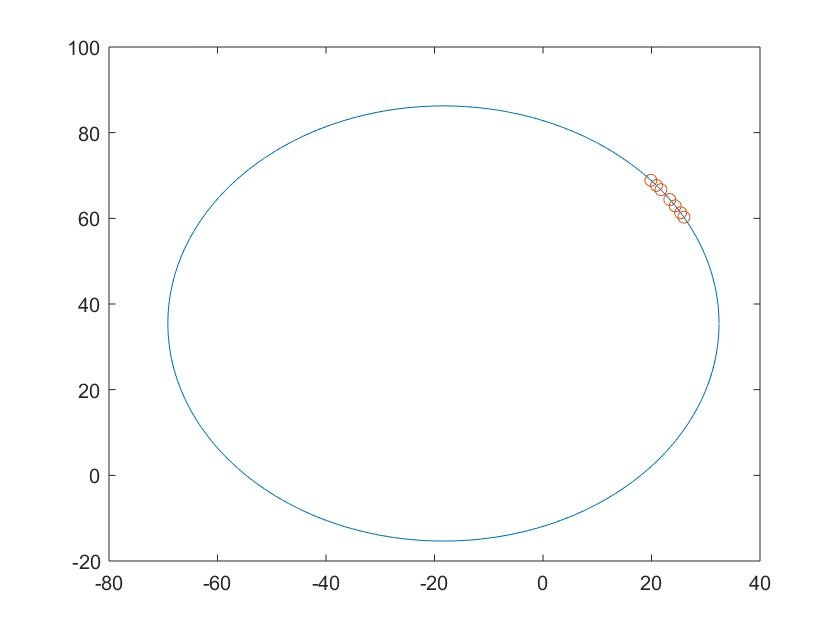
\includegraphics[width=9cm]{leastSq.jpg}
\end{figure}

\end{outputs}

\end{sol}








% 7.9
\section{Orthonormal Bases and the Gram Schmidt Process}

\begin{exer} (\textit{Gram-Schmidt Process})\\
Perform the Gram-Schmidt process to transform the vectors given in the Example 9 of the Section 7.9 to obtain an orthonormal basis for $\mathbb{R}^{3}$.

In this problem, use a nested loop and the MATLAB command \textit{norm}.
\end{exer}

\begin{sol}

\begin{verbatim}

w1 = [1 1 1]'; w2 = [0 1 1]'; w3 = [0 0 1]';
A = [w1 w2 w3]; % Construct a matrix A whose columns are w1, w2, and w3.
format short; [m, n] = size(A);
Q = zeros(m, n); % Initialize the matrix Q as an m*n zero matrix.

% Find an orthonormal basis for the column space of A.
for j = 1 : n
    v = A(:, j); % v begins as jth column of A.
    for i = 1 : (j-1)
        temp = Q(:, i)' * A(:, j);
        % Subtract each component of orthogonal projection of v
        % onto the subspace spanned by the vector Q(:, i).
        v = v - temp * Q(:, i);
    end
    Q(:, j) = v / norm(v); % Normalize v by its 2-norm.
end
disp('The orthonormal basis {q1,q2,q3} for R^3 from {w1,w2,w3} are as follows:')
disp('q1='); disp(Q(:,1)'); disp('q2='); disp(Q(:,2)'); disp('q3='); disp(Q(:,3)');
\end{verbatim}

\begin{outputs}
\begin{verbatim}

The orthonormal basis {q1,q2,q3} for R^3 from {w1,w2,w3} are as follows:
q1=
    0.5774    0.5774    0.5774

q2=
   -0.8165    0.4082    0.4082

q3=
   -0.0000   -0.7071    0.7071
\end{verbatim}
\end{outputs}

\end{sol}

\vspace{3mm}
\begin{exer}\label{GS} (\textit{Orthonormal Bases for the Four Fundamental Spaces})\\
Find orthonormal bases for the four fundamental spaces of the matrix


\begin{displaymath}
A = \left[\begin{array}{rrrr} 2& \hspace{2mm} -1& \hspace{5mm} 3&\hspace{4mm} 5\\ 4 & -3 & 1 & 3 \\ 3 & -2 & 3 & 4 \\ 4 & -1 & 15 & 17 \\ 7 & -6 & -7 & 0  \end{array} \right].
\end{displaymath}
\end{exer}

\begin{sol}

\begin{verbatim}

%--- The following is the function file 'GramSchmidt.m'. ---%

% Find an orthonormal basis for col(A) when A has full column rank.
function Q = GramSchmidt(A)

  [m, n] = size(A);

  % Initialize the matrix Q as an m*n zero matrix.
  Q = zeros(m, n); 

  for j = 1 : n
    % v begins as jth column of A.
    v = A(:, j); 
    for i = 1 : (j-1)
      temp = Q(:, i)' * A(:, j);
      % Subtract each component of orthogonal projection of v
      % onto the subspace spanned by the vector Q(:, i).
      v = v - temp * Q(:, i);
    end
    Q(:, j) = v / norm(v); % Normalize v by its 2-norm.
  end
end
% Q is an m*n matrix whose columns form an orthonormal basis for col(A).
\end{verbatim}

The following commands are performed in the command window of MATLAB.

\begin{verbatim}
A = [2 -1 3 5; 4 -3 1 3; 3 -2 3 4; 4 -1 15 17; 7 -6 -7 0];
format short;

% Find the reduced row echelon form of A.
rref_A = rref(A); 

% (1). Find an orthonormal basis for the row space of A.
% From the result of rref_A, the first three nonzero rows in rref_A form
% a basis for the row space of A.

% Construct a matrix R_A whose columns are a basis for the row space of A.
R_A = rref_A(1:3, :)';

% Find an orthonormal basis for the column space of R_A by Gram-Schmidt process,
% which is the same as finding an orthonormal basis for the row space of A.
Orth_R_A = GramSchmidt(R_A);

a1 = Orth_R_A(:, 1); a2 = Orth_R_A(:, 2); a3 = Orth_R_A(:, 3);

disp('An orthonormal basis {a1, a2, a3} for the row space of A is');
disp('a1 = '); disp(a1'); disp('a2 = '); disp(a2'); disp('a3 = '); disp(a3');

% (2). Find an orthonormal basis for the column space of A.
% From the result of rref_A, the first three columns of A are the pivot columns
% which form a basis for the column space of A.

% Construct a matrix C_A whose columns are a basis for the column space of A.
C_A = A(:, 1:3);

% Find an orthonormal basis for the column space of C_A by Gram-Schmidt process,
% which is the same as finding an orthonormal basis for the column space of A.
Orth_C_A = GramSchmidt(C_A);

b1 = Orth_C_A(:, 1); b2 = Orth_C_A(:, 2); b3 = Orth_C_A(:, 3);

disp('An orthonormal basis {b1, b2, b3} for the column space of A is');
disp('b1 = '); disp(b1'); disp('b2 = '); disp(b2'); disp('b3 = '); disp(b3');


% (3). Find an orthonormal basis for the null space of A.
% In addition, from the result of rref_A,
% we can easily see that {[-6 -7 0 1]'} is a basis for N(A).

% Construct a matrix N_A whose columns are a basis for the null space of A.
N_A = [-6 -7 0 1]';

% Find an orthonormal basis for the column space of N_A by Gram-Schmidt process,
% which is the same as finding an orthonormal basis for the null space of A.
Orth_N_A = GramSchmidt(N_A);

c1 = Orth_N_A(:, 1);
disp('An orthonormal basis {c1} for the null space of A is');
disp('c1 = '); disp(c1');

% (4). Find an orthonormal basis for the null space of A transpose.
[L U P] = lu(A);
temp = [0 0 0 0 1]';
\% Make L a square matrix of order 5.
L = [L temp]; 

% Make U have the same size of A.
U(5, :) = 0; 

% Then, we have P*A = L*U, which is the same result as above.
% Note that L^(-1)*P*A = U, where U is an upper triangular matrix.

E = L^(-1)*P;

% Since E = L^(-1)*P is a product of elementary matrices s.t. E*A=U,
% E represents a set of elementary row operations
% that makes A become a row echelon form U.

% ref_par_A is the resulting partitioned matrix [U E].
ref_par_A = [U E]; 

% From the result of ref_par_A, we can see that ref_par_A([4:5], [1:4]) = 0.
% Thus, the row vectors of E2 form a basis for null(A'),
% where E2 = ref_par_A([4:5], [5:9]).

% Construct a matrix N_Atrans whose columns are a basis for
% the null space of A transpose.
N_Atrans = ref_par_A(4:5, 5:9)';

% Find an orthonormal basis for the column space of N_Atrans by Gram-Schmidt process,
% which is the same as finding an orthonormal basis for the null space of A transpose.
Orth_N_Atrans = GramSchmidt(N_Atrans);

d1 = Orth_N_Atrans(:, 1); d2 = Orth_N_Atrans(:, 2);
disp('An orthonormal basis {d1, d2} for the null space of the transpose of A is');
disp('d1 = '); disp(d1'); disp('d2 = '); disp(d2');
\end{verbatim}

\begin{outputs}
\begin{verbatim}

An orthonormal basis {a1, a2, a3} for the row space of A is
a1 =
    0.1644         0         0    0.9864

a2 =
   -0.7446    0.6559         0    0.1241

a3 =
     0     0     1     0

An orthonormal basis {b1, b2, b3} for the column space of A is
b1 =
    0.2063    0.4126    0.3094    0.4126    0.7220

b2 =
    0.1873   -0.0887    0.0493    0.8378   -0.5027

b3 =
   -0.3699    0.5812    0.5878   -0.1321   -0.4029

An orthonormal basis {c1} for the null space of A is
c1 =
   -0.6470   -0.7548         0    0.1078

An orthonormal basis {d1, d2} for the null space of the transpose of A is
d1 =
    0.8649    0.3089         0   -0.3089   -0.2471

d2 =
    0.1936   -0.6234    0.7458   -0.1224    0.0512
\end{verbatim}
\end{outputs}

\end{sol}






% section 7.10


\section{$QR-$Decomposition; Householder Transformations}


\begin{exer}(\textit{$QR-$Decomposition})\\
\begin{enumerate}
\item[(a)] Make a function file \verb"myQR.m" to find a $QR$-decomposition of a given matrix. 
You may use your function file \verb"GS_process.m" from the \textbf{Exercise}~\ref{GS}.
\vspace{1mm}
\item[(b)] $$A=\begin{bmatrix} 1 & 1 & 1\\ 1& 0 & 2\\ 0 & 1& 2\end{bmatrix}.$$
Compare your result with the output produced by the MATLAB command \textit{qr}. 
\end{enumerate}
\end{exer}


\begin{sol}
\begin{verbatim}

%(a)
%--- This is a function file myQR.m ---%

function [Q R]=myQR(A)
 Q=GS_process(A);
 R=Q'*A;
end

%(b)
A=[1 1 1; 1 0 2; 0 1 2];
[Q1 R1]=myQR(A); [Q R]=qr(A);

disp('my QR result'); disp('Q');disp(Q1); disp('R');disp(R1);
disp('MATLAB QR result'); disp('Q');disp(Q); disp('R');disp(R);
\end{verbatim}

\begin{outputs}
\begin{verbatim}

my QR result
Q
    0.7071    0.4082   -0.5774
    0.7071   -0.4082    0.5774
         0    0.8165    0.5774
R
    1.4142    0.7071    2.1213
    0.0000    1.2247    1.2247
    0.0000   -0.0000    1.7321

MATLAB QR result
Q
   -0.7071    0.4082   -0.5774
   -0.7071   -0.4082    0.5774
         0    0.8165    0.5774
R
   -1.4142   -0.7071   -2.1213
         0    1.2247    1.2247
         0         0    1.7321
\end{verbatim}

\end{outputs}


\noindent The results are the same.
\end{sol}







% 7.11

\section{Coordinates with Respect to a Basis}

\begin{exer} (\textit{Transition Matrices between Two Different Bases})\\

\begin{enumerate}

\item[(a)] Confirm that $B_{1} = \{\mathbf{u}_{1}, \mathbf{u}_{2}, \mathbf{u}_{3}, \mathbf{u}_{4}, \mathbf{u}_{5}\}$ and $B_{2} = \{\mathbf{v}_{1}, \mathbf{v}_{2}, \mathbf{v}_{3}, \mathbf{v}_{4}, \mathbf{v}_{5}\}$ are bases for $\mathbb{R}^{5}$, and find the transition matrices $P_{\tiny{B_{1} \rightarrow B_{2}}}$ and $P_{\tiny{B_{2} \rightarrow B_{1}}}$, where

\begin{displaymath}
\begin{array}{lllllll}
\vspace{1mm} \mathbf{u}_{1} & = & (3, \hspace{1mm} 1, \hspace{1mm} 3, \hspace{1mm} 2, \hspace{1mm} 6) & \hspace{4mm} & \mathbf{v}_{1} & = & (2, \hspace{1mm} 6, \hspace{1mm} 3, \hspace{1mm} 4, \hspace{1mm} 2) \\ \vspace{1mm} \mathbf{u}_{2} & = & (4, \hspace{1mm} 5, \hspace{1mm} 7, \hspace{1mm} 2, \hspace{1mm} 4) & \hspace{4mm} & \mathbf{v}_{2} & = & (3, \hspace{1mm} 1, \hspace{1mm} 5, \hspace{1mm} 8, \hspace{1mm} 3) \\ \vspace{1mm} \mathbf{u}_{3} & = & (3, \hspace{1mm} 2, \hspace{1mm} 1, \hspace{1mm} 5, \hspace{1mm} 4) & \hspace{4mm} & \mathbf{v}_{3} & = & (5, \hspace{1mm} 1, \hspace{1mm} 2, \hspace{1mm} 6, \hspace{1mm} 7) \\ \vspace{1mm} \mathbf{u}_{4} & = & (2, \hspace{1mm} 9, \hspace{1mm} 1, \hspace{1mm} 4, \hspace{1mm} 4) & \hspace{4mm} & \mathbf{v}_{4} & = & (8, \hspace{1mm} 4, \hspace{1mm} 3, \hspace{1mm} 2, \hspace{1mm} 6) \\ \vspace{1mm} \mathbf{u}_{5} & = & (3, \hspace{1mm} 3, \hspace{1mm} 6, \hspace{1mm} 6, \hspace{1mm} 7) & \hspace{4mm} & \mathbf{v}_{5} & = & (5, \hspace{1mm} 5, \hspace{1mm} 6, \hspace{1mm} 3, \hspace{1mm} 4) \\
\end{array}
\end{displaymath}



\item[(b)] Find the coordinate matrices with respect to $B_{1}$ and $B_{2}$ of $\mathbf{w} = (1, \hspace{1mm} 1, \hspace{1mm} 1, \hspace{1mm} 1, \hspace{1mm} 1)$.

\end{enumerate}

\end{exer}



\begin{sol}
\begin{verbatim}

u1 = [3 1 3 2 6]'; v1 = [2 6 3 4 2]';
u2 = [4 5 7 2 4]'; v2 = [3 1 5 8 3]';
u3 = [3 2 1 5 4]'; v3 = [5 1 2 6 7]';
u4 = [2 9 1 4 4]'; v4 = [8 4 3 2 6]';
u5 = [3 3 6 6 7]'; v5 = [5 5 6 3 4]';

U = [u1 u2 u3 u4 u5]; 
V = [v1 v2 v3 v4 v5]; 

format short;

% Initialization.
P_B1B2 = zeros(5); 
P_B2B1 = zeros(5); 

for j = 1:5
  % Find the coordinate vector of U(:, j) in B1 with respect to B2.
  P_B1B2(:, j) = V\U(:, j);
  % Find the coordinate vector of V(:, j) in B2 with respect to B1.
  P_B2B1(:, j) = U\V(:, j);
end

disp('The transition matrix from B1 to B2 is'); disp(P_B1B2);
disp('The transition matrix from B2 to B1 is'); disp(P_B2B1);

w = [1 1 1 1 1]';

% Find the coordinate matrix of w with respect to B1.
w_B1 = U\w; 

% Find the coordinate matrix of w with respect to B2.
w_B2 = P_B1B2 * w_B1; 

disp('The coordinate matrix of w with respect to B1 is'); disp(w_B1');
disp('The coordinate matrix of w with respect to B2 is'); disp(w_B2');
\end{verbatim}


\begin{outputs}
\begin{verbatim}

The transition matrix from B1 to B2 is
   -0.4992   -0.2531    0.4843    1.8286   -0.2123
   -0.7830   -0.3679    0.1604   -0.8019   -0.5849
    1.3019    0.2925    0.4623    0.6887    1.4906
   -0.9096   -0.6116    0.1918   -0.2091   -1.4104
    1.4230    1.8082   -0.4591   -0.2044    1.8019

The transition matrix from B2 to B1 is
   -0.6889   -1.3556    0.6222    1.2667   -0.0444
    0.4067    0.3591    0.0278    1.2083    1.0873
    0.3151    1.2675    1.3444    1.6833    0.6540
    0.3615   -0.5433   -0.2056   -0.1417   -0.0746
    0.2571    0.9714   -0.2000   -1.8000   -0.3429

The coordinate matrix of w with respect to B1 is
   -0.0222    0.1508    0.1841   -0.0016   -0.0286

The coordinate matrix of w with respect to B2 is
    0.0653    0.0094    0.0566    0.0039    0.1053
\end{verbatim}
\end{outputs}

\end{sol}
